%%%%%%%%%%%%%%%%%%%%%%%%%%%%%%%%%%%%%%%%%%%%%%%%%%%%%%%%%%%%%%%%%%%%%%%
%%%%%%%%%%%%%%%%%%%%%%%%%%%%%%%%%%%%%%%%%%%%%%%%%%%%%%%%%%%%%%%%%%%%%%%
%%%%%                                                                 %
%%%%%     <file_name>.tex                                             %
%%%%%                                                                 %
%%%%% Author:      <author>                                           %
%%%%% Created:     <date>                                             %
%%%%% Description: <description>                                      %
%%%%%                                                                 %
%%%%%%%%%%%%%%%%%%%%%%%%%%%%%%%%%%%%%%%%%%%%%%%%%%%%%%%%%%%%%%%%%%%%%%%
%%%%%%%%%%%%%%%%%%%%%%%%%%%%%%%%%%%%%%%%%%%%%%%%%%%%%%%%%%%%%%%%%%%%%%%

\chapter{Control System Implementation}

The software for the micro-controller was implemented using the C Programming Language. I considered using a real-time operating system but decided that in this case it would be simpler to not to do so. The software runs a main loop and all modules are fundamentally asynchronous. In testing it was possible to show that this yielded very good performance.

Another major design decision is to use only static memory allocation. Although at times this can be limiting and is less space efficient than dynamic memory allocation, it also leads to higher performance. More importantly, this approach guarantees that there are no memory leaks, which can otherwise become fatal bugs that may be difficult to diagnose.

\section{Structure}

Each CPU core runs independently from the other, except during system initialisation. Since some peripherals need to be initialised in the correct sequence and the main loop should not be entered until the entire system is initialised, inter-processor communication (IPC) flags are used to synchronise both cores during start-up.

Each core has dedicated FLASH memory, as well as dedicated RAM regions. Additional shared RAM can be read by both CPUs but only written to by one CPU per block. At boot CPU1 configures the global shared RAM regions according to the applications needs and then sends a command to the boot loader on CPU2 using IPC registers to start the program for CPU2.

\begin{figure}[H]
    \centering 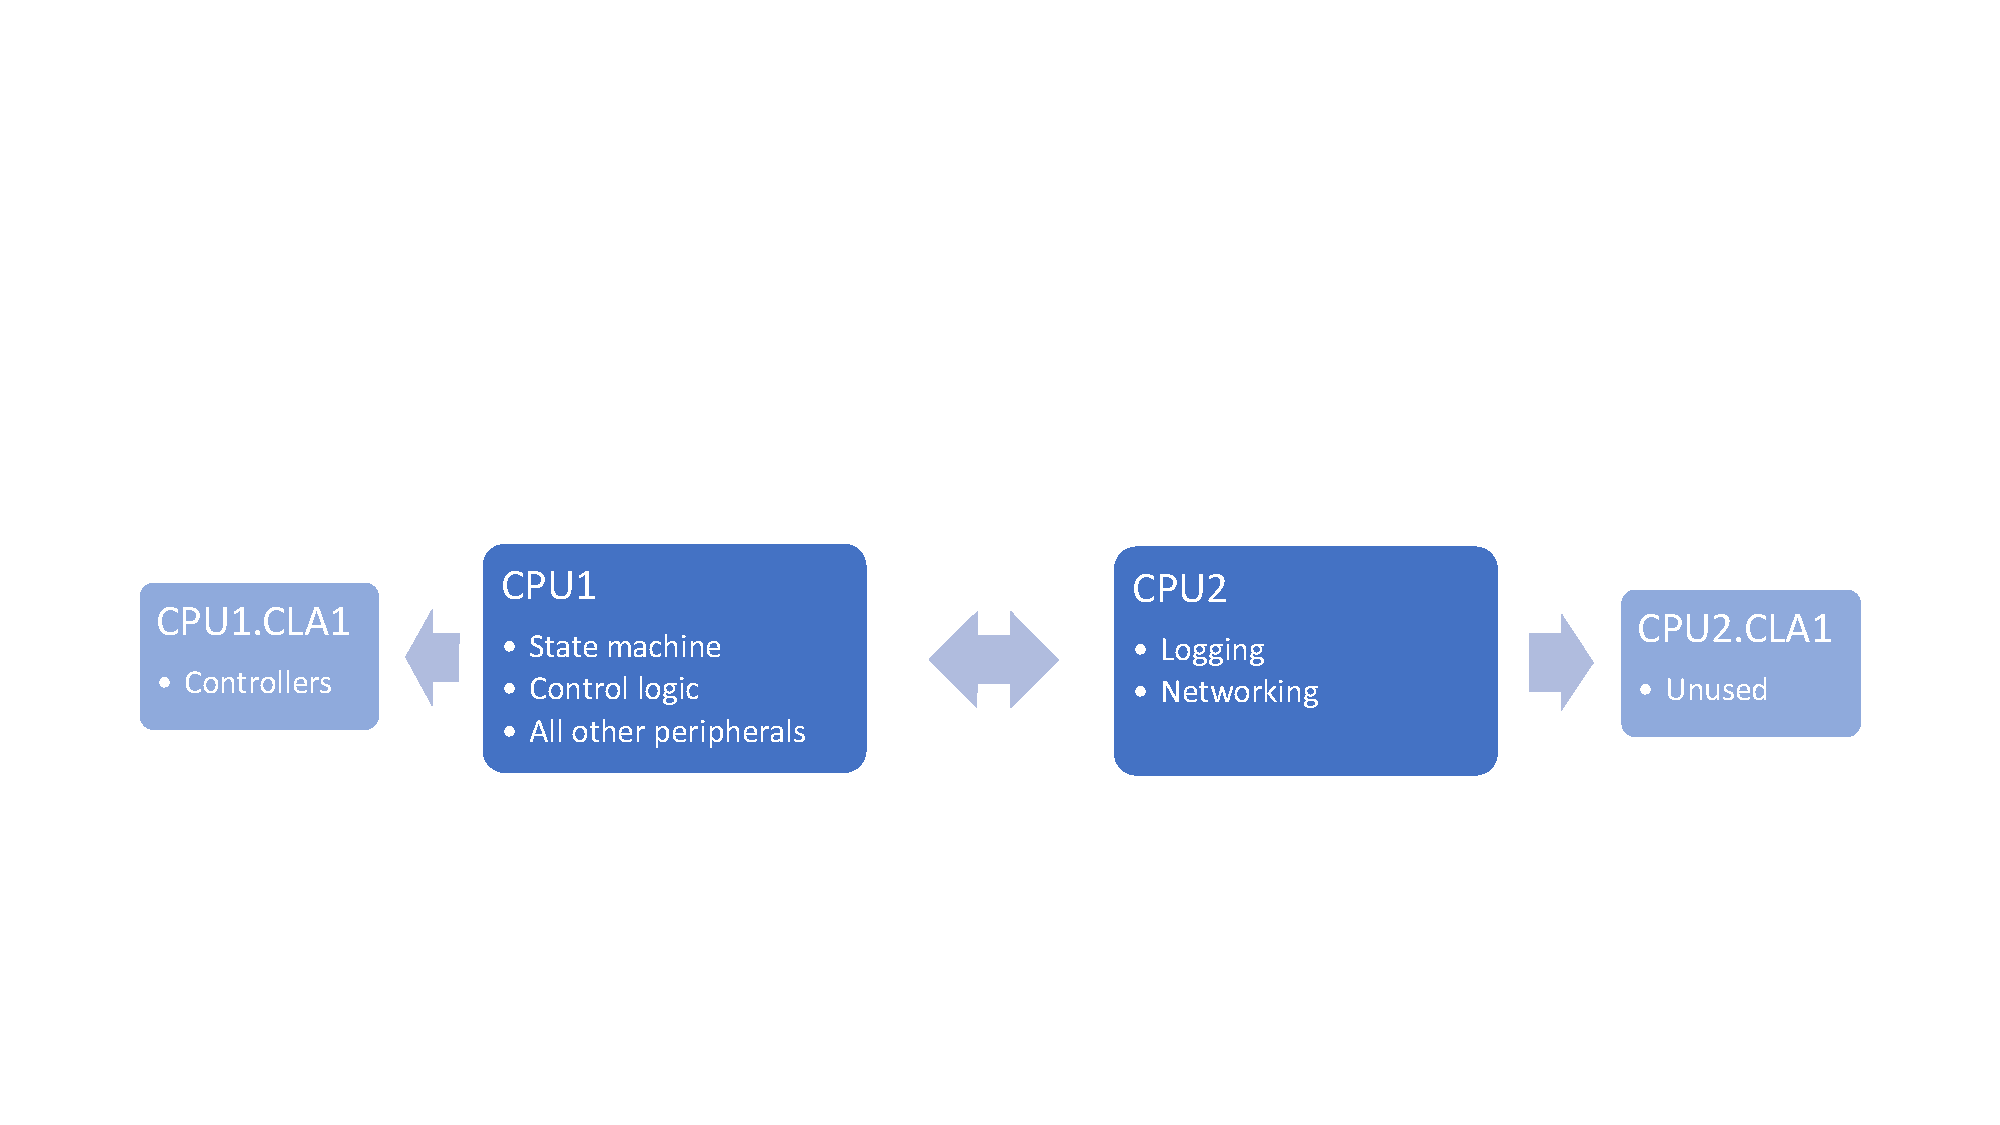
\includegraphics[width=1.0\textwidth]{./figures/system_structure.pdf}
    \caption{Division of tasks between processors and co-processors.}
    \label{fig:system_structure}
\end{figure}

Figure~\ref{fig:system_structure} shows the division of tasks between the two CPU cores and one of the Control Law Accelerator (CLA) co-processors. CPU runs most drivers and handles the control logic and state machine. All sensor data is processed on this core and all control decisions are made on it as well. This consolidates the data processing and control logic in one program with out the need for concurrency control that could be subject to hard to find bugs.

CPU2 is dedicated to Logging and Networking. The main constraint for this is that the FAT file system is computationally heavy and as will be discussed in section~\ref{logging} is hard to implement asynchronously. In order to reduce the performance impact, logging was separated onto the second core. However, since the Ethernet controller uses the same SPI bus as the SD-card and only one CPU core can be the master of each peripheral (in this case one of the SPI interfaces), networking also needs to be handled on the second core.

The traction and yaw controllers must run regularly in precise intervals and therefore somewhat contradict the asynchronous nature of the remaining system. Furthermore, as they were developed by other people who did not necessarily have detailed knowledge of the system, it made sense to provide an isolated environment for the execution of the controllers.

The CLA co-processor runs at the same frequency as the associated CPU core but executes code independently. It is assigned areas of the associated CPU's dedicated RAM for program and data space. As the CLA co-processor is designed to run controllers, it can be assigned up to eight function pointers, which represent tasks. These tasks can be triggered from peripherals but also from software running on the CPU. Once a task is triggered, it runs to completion. Although the instruction set for the CLA is separate and significantly more limited, these other features make the CLA perfectly suited for the task.

\subsection{Module life-cycle}

All modules and drivers follow a similar structure. This structure mainly consists of three functions that are called at different times during the module life-cycle as illustrates in Figure~\ref{fig:module_lifecycle}: \mintinline{c}{init()}, \mintinline{c}{configure()} and \mintinline{c}{update()}.

\begin{figure}[H]
    \centering 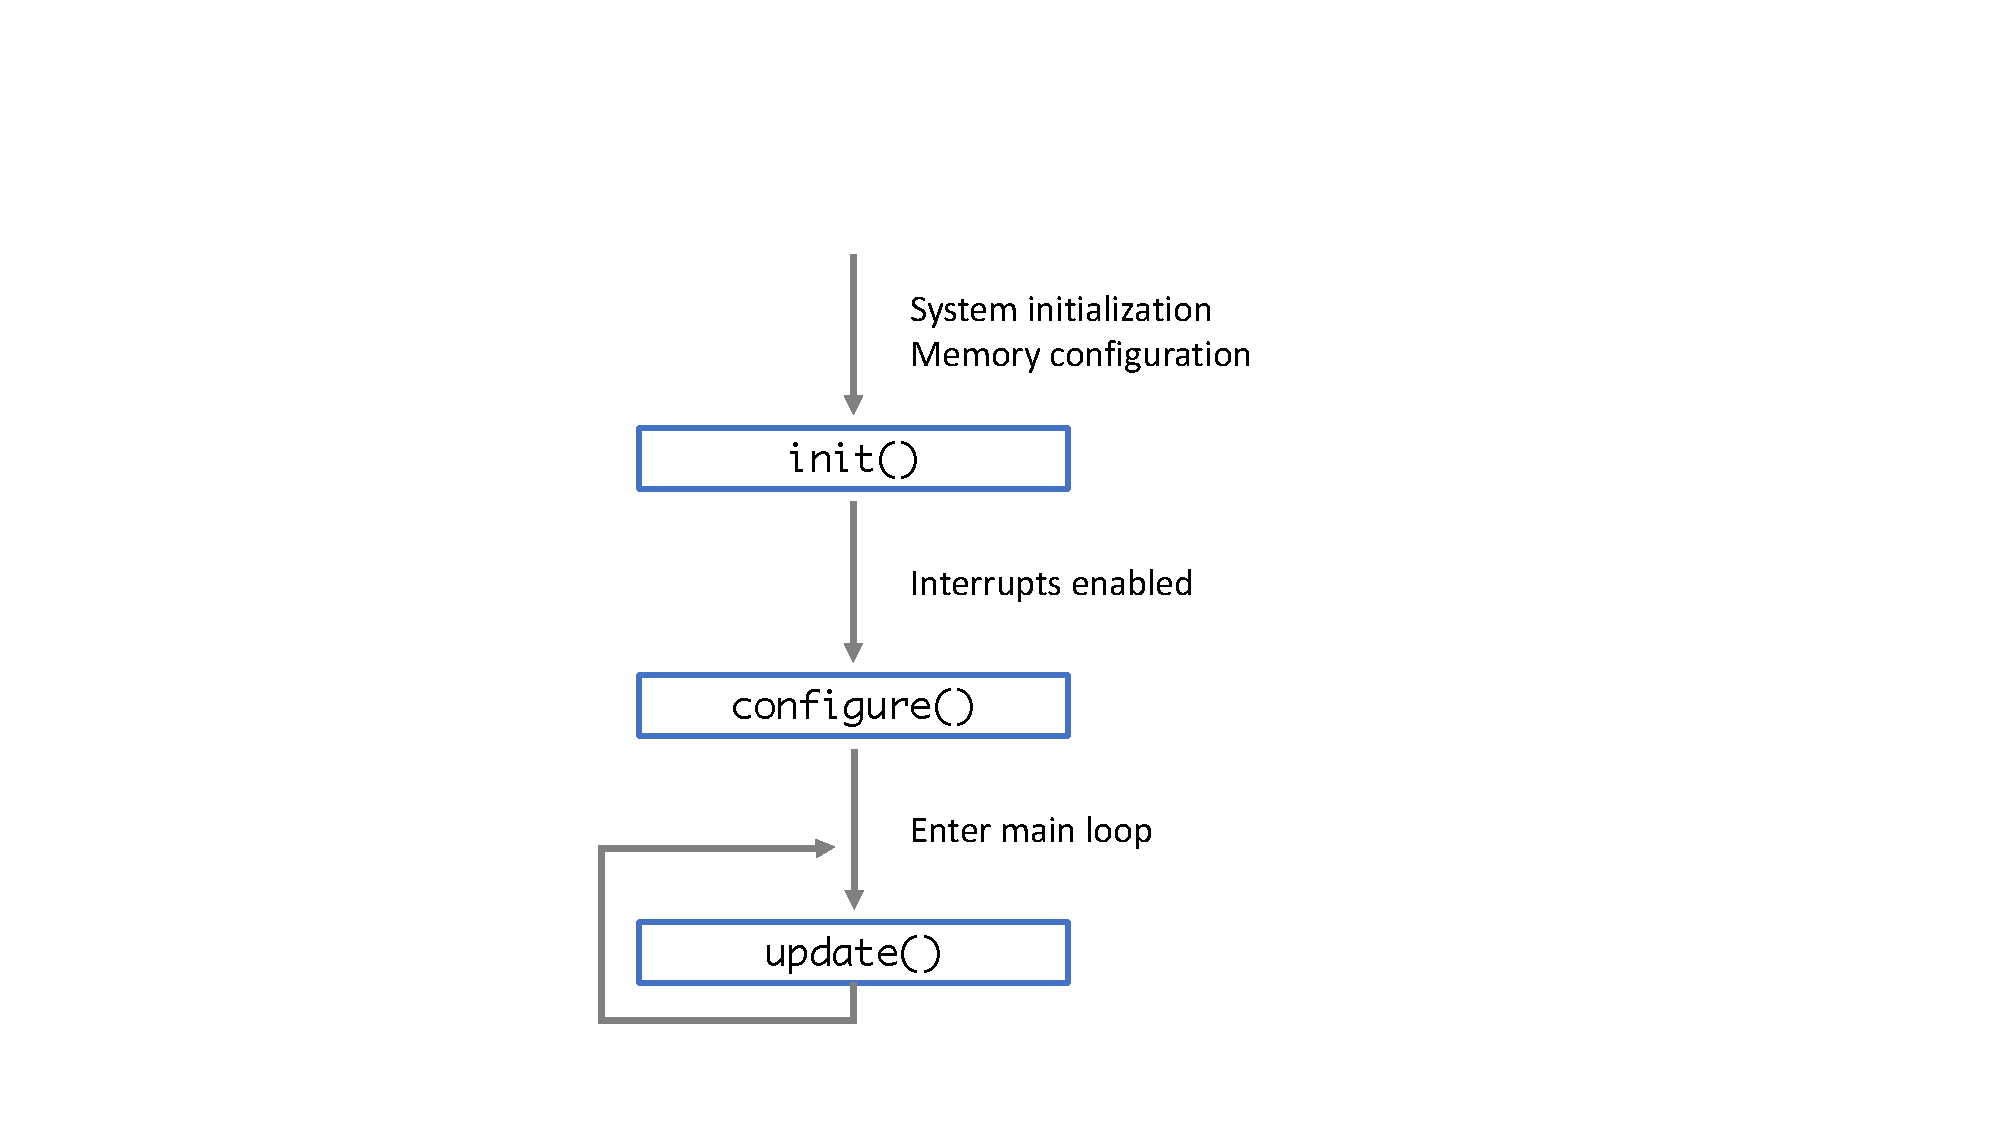
\includegraphics[width=0.5\textwidth]{./figures/module_lifecycle.pdf}
    \caption{Life-cycle of each module in the system.}
    \label{fig:module_lifecycle}
\end{figure}

Immediately after system initialization and memory configuration is complete, \mintinline{c}{init()} is called to allow modules to perform initialisation routines, configure peripherals and enable required interrupts. However, interrupts remain globally disabled for the duration of these function's execution.

Some drivers require further initialisation after interrupts have been enabled. Mostly this involves the configuration of an external device such as the Ethernet Controller, SD-card and laser distance sensors. For these initialisation sequences require fully functional communication and therefore interrupts. This is the purpose of the \mintinline{c}{configure()} functions.

After start-up is complete the processor enters the main loop. At each iteration of the loop the \mintinline{c}{update()} function of each module is called. If the module does not need to perform any computation at that time it immediately returns. Several modules use internal finite state machines in order to allow for asynchronous execution.

\subsection{Data-flow}

\begin{figure}[H]
    \centering 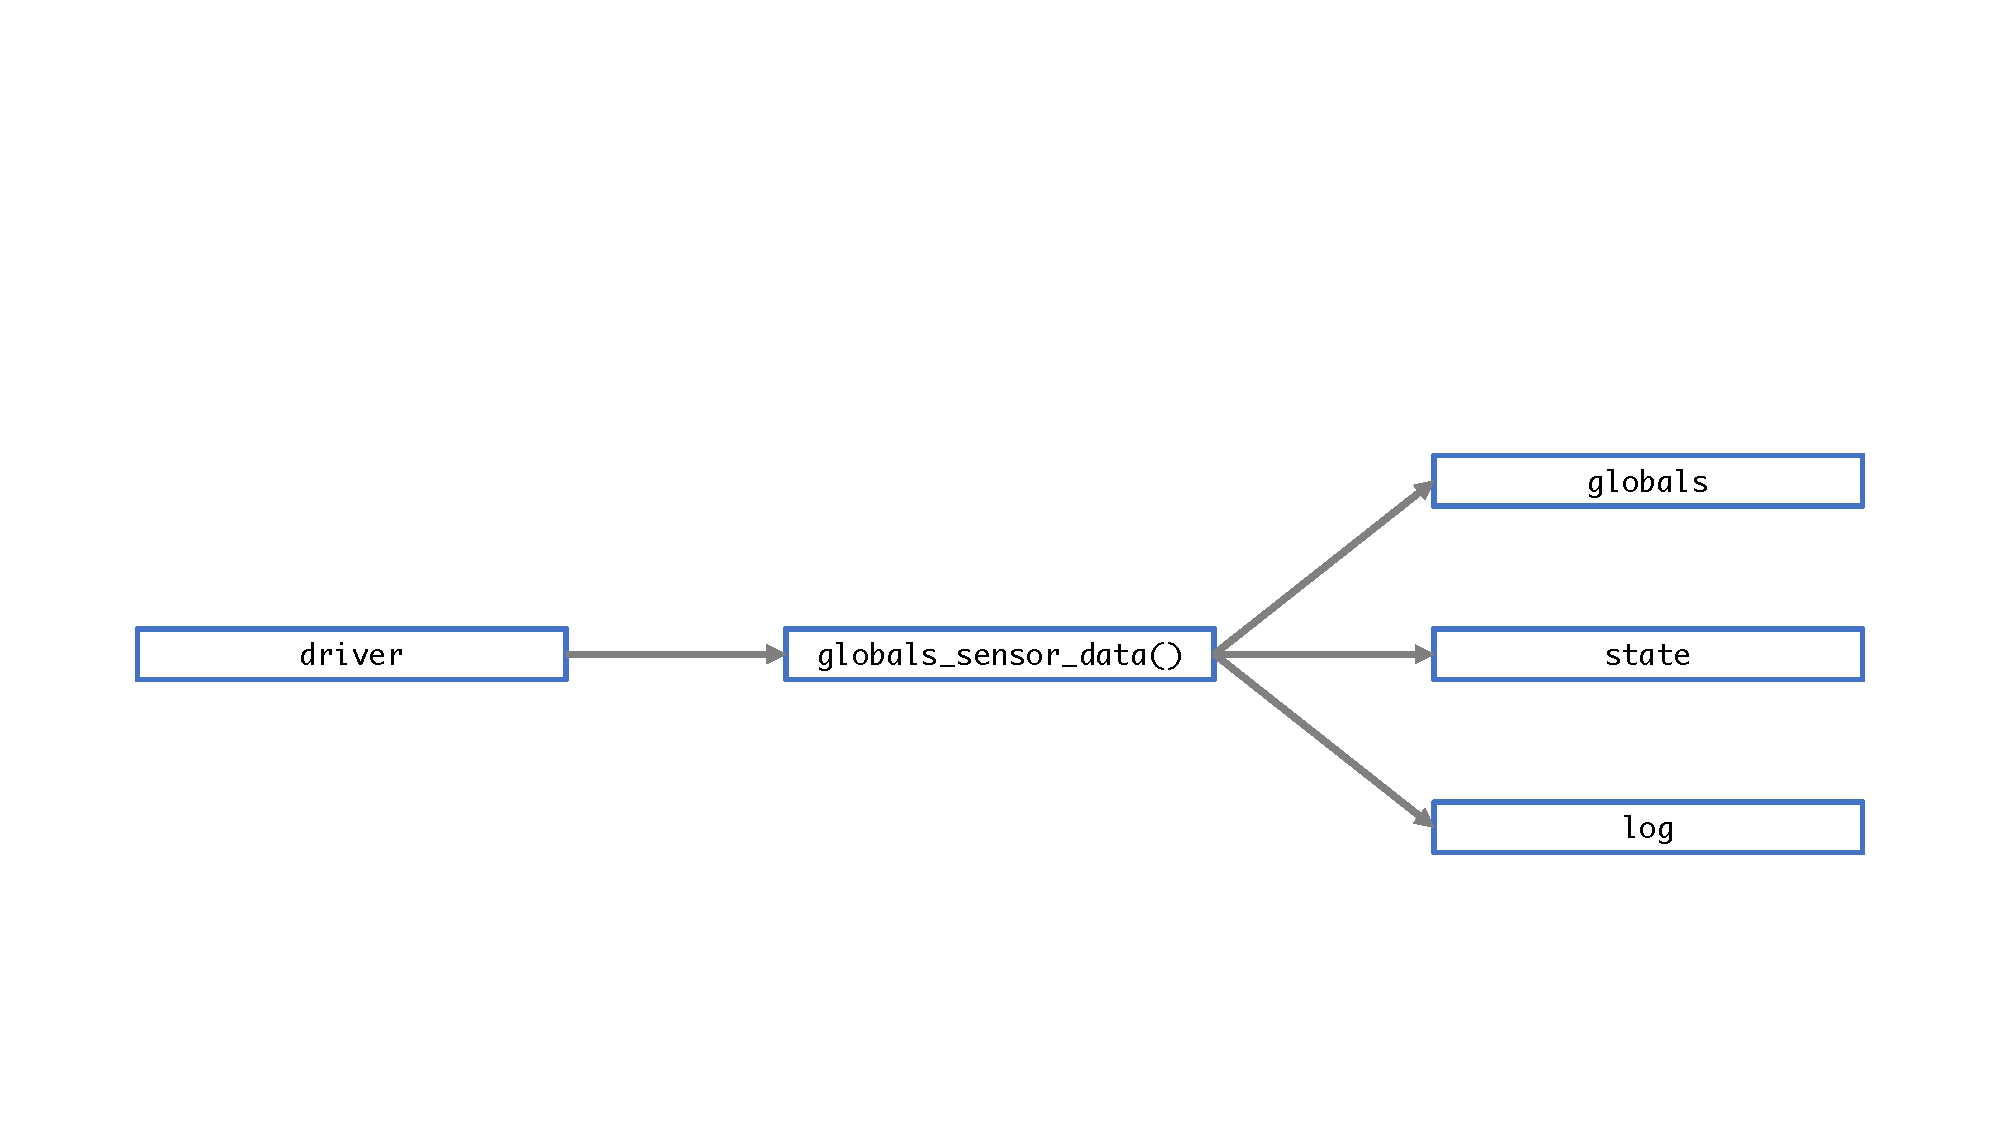
\includegraphics[width=1.0\textwidth]{./figures/dataflow.pdf}
    \caption{Flow of sensor data and derived data.}
    \label{fig:dataflow}
\end{figure}

All data processing is centralised using the \mintinline{c}{globals_sensor_data()} function. The concept is to simplify how data is distributed throughout the program. Drivers call \mintinline{c}{globals_sensor_data()} whenever a new data point is gathered from a sensor. Derived data such as velocity or location is also collected through this function. In this way the data flow is abstracted from the driver layer improving modularisation, maintainability and flexibility.

Once a data point has been collected by a call to \mintinline{c}{globals_sensor_data()}, the data can be stored to a global structure for use by other modules and used to to update the global finite state machine. Additionally, all data points are logged as will be described in Section~\ref{logging}.

\section{Networking}

The network protocol needs to be resistant to packet loss and unstable network connections, while still providing a steady stream of data. Unlike the event-based logging system (Section~\ref{logging}) telemetry data transmitted over the network can be relatively infrequent and there is no data that must be delivered at a higher rate than other data. Therefore I implemented the protocol using UDP packets. The structure listed in Appendix~\ref{telemetry_frame} holds all the data that needs to be transmitted. It fits into a single UDP packet without segmentation. This makes it very efficient to transmit telemetry and resistant to occasional packet loss as only one packet is needed to observe the pod's state.

For controlling the pod remotely from the control panel the protocol follows an analogous scheme using a control frame consisting of the following structure.

\begin{minted}{c}
struct ctrl_frame {
    uint16_t set_state;     // 0: D.C. / ..: the state
    uint16_t aux_power;     // 0: D.C. / 1: OFF / 2: ON
    uint16_t precharge;     // 0: D.C. / 1: OFF / 2: ON
    uint16_t battery;       // 0: D.C. / 1: OFF / 2: ON
    uint16_t brakes;        // 0: D.C. / 1: DISENGAGE / 2: ENGAGE
    uint16_t low_speed;     // 0: D.C. / 1: BACK / 2: STOP / 3: FWD
    uint16_t clear_fault;   // 0: D.C. / 1: CLEAR
    uint16_t reset_run;     // 0: D.C. / 1: RESET
    uint16_t bms_power;     // 0: D.C. / 1: OFF / 2: ON
    uint16_t eject_sd_card; // 0: D.C. / 1: EJECT
};
\end{minted}

Both the telemetry frame and control frame must be sent (and received) regularly in order for the pod and the control panel to check connectivity and enter a safe state should it fail. Therefore the fields in the control frame are usually zero and a non-zero value indicates a control command.

Although the networking drive primarily executes on CPU2, a small portion also executes on CPU1. This is necessary, since all telemetry data originates from CPU1. Rather than placing data in global structures unnecessarily, the telemetry frame is simply assembled on CPU1 and then read by the DMA controller on CPU2. Similarly, CPU2 receives incoming control packets and CPU1 decodes them and executes any control commands. This process is illustrated by Figure~\ref{fig:networking_structure}.

\begin{figure}[H]
    \centering 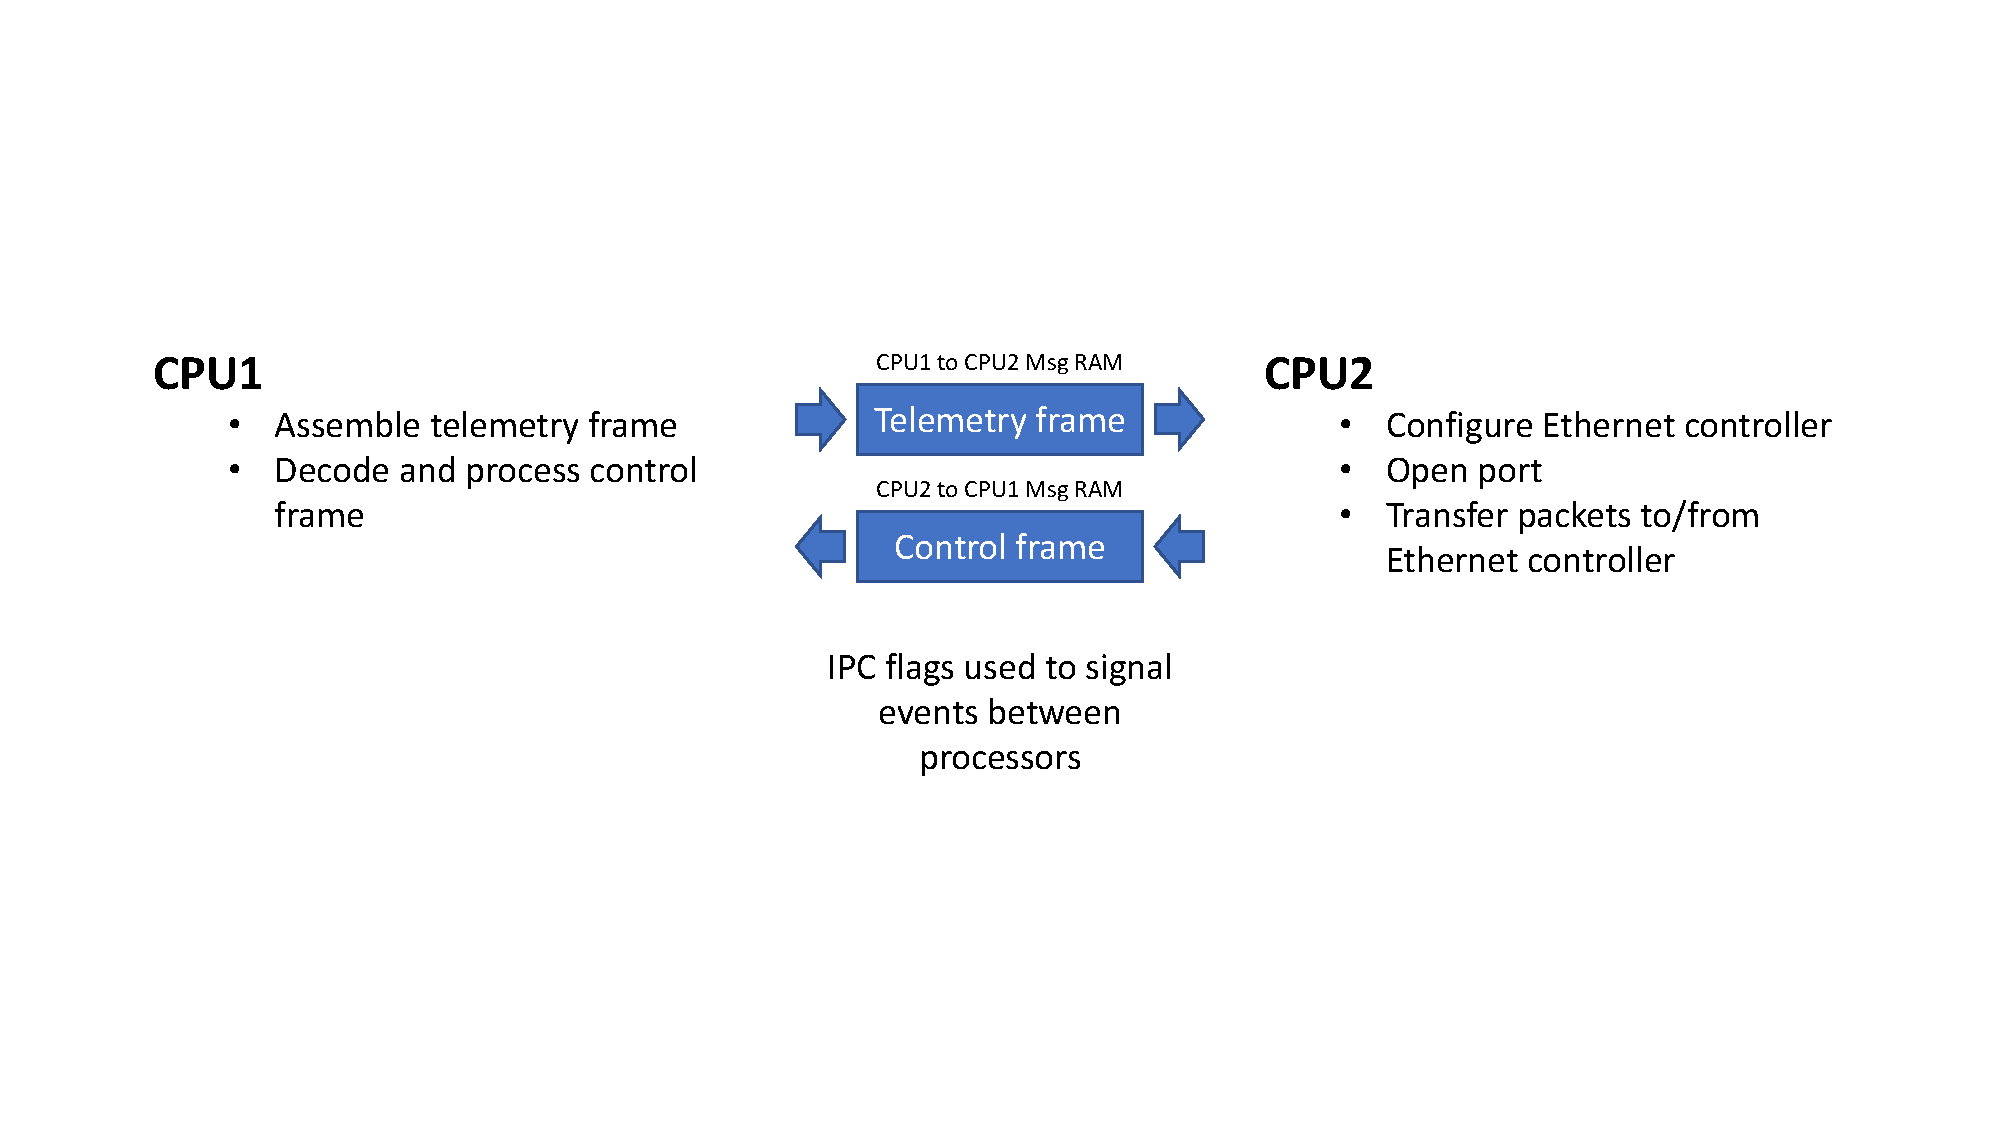
\includegraphics[width=1.0\textwidth]{./figures/networking_structure.pdf}
    \caption{Structure of networking driver.}
    \label{fig:networking_structure}
\end{figure}

The telemetry and control frames are written to Message RAM, which is a shared memory area specifically designed for this kind of usage. It consists of two 1K regions, one writeable only by CPU1 and one only writeable by CPU2. The telemetry frame only consists of 76 16-bit words and therefore easily fits into the Message RAM. The micro-controllers Interprocessor Communication (IPC) module further provides flag registers. The networking driver uses IPC flags to notify the other CPU of the following events:

\begin{itemize}
    \item CPU1 $\rightarrow$ CPU2: Telemetry frame assembled and ready for transmission.
    \item CPU2 $\rightarrow$ CPU1: Telemetry frame has been transmitted and can be overwritten.
    \item CPU2 $\rightarrow$ CPU1: Control frame received.
    \item CPU1 $\rightarrow$ CPU2: Control frame has been processed and can be overwritten.
\end{itemize}

To achieve the highest possible performance all SPI communication with the Ethernet controller is implemented using the micro-controller's DMA controller. Since the SPI interface can be used with a 16-level FIFO extension, the DMA controller can operate in Burst mode. This means that the data is transferred in bursts of 16 words until the transfer has completed. The next bust is triggered by the FIFO interrupt which can be configured to assert at a specific level. For this implementation it is configured to trigger when the FIFO is empty but depending on the size of the bursts this can be optimized.

The following listing shows the process of configuring channel one of the DMA controller for transmission of a buffer at \mintinline{c}{src} of length \mintinline{c}{len}. Notice that the burst length must be a divisor of the total buffer size. This is because the DMA controller cannot handle bursts of different lengths.

\begin{minted}{c}
void spia_tx_dma(uint16_t *src, uint16_t len)
{
    uint16_t burst;

    // Calculate largest burst length
    for (burst = 16; len % burst; burst /= 2) ;

    // Reset the TX FIFO
    SpiaRegs.SPIFFTX.bit.TXFIFO = 0;

    // Configure DMACH1 for SPIA TX
    DMACH1AddrConfig(&SpiaRegs.SPITXBUF, src);
    DMACH1BurstConfig(burst - 1, 1, 0);             // Burst size, src step, dest step
    DMACH1TransferConfig((len / burst) - 1, 1, 0);  // Number of transfers, src step, dest step
    DMACH1ModeConfig(DMA_SPIATX,PERINT_ENABLE,ONESHOT_DISABLE,CONT_DISABLE,
                     SYNC_DISABLE,SYNC_SRC,OVRFLOW_DISABLE,SIXTEEN_BIT,
                     CHINT_END,CHINT_ENABLE);

    // Set the TX FIFO interrupt level
    SpiaRegs.SPIFFTX.bit.TXFFIL = 0;

    // Start the DMA transfer
    _spia_tx_dma_done = 0;
    StartDMACH1();

    // Release the TX FIFO from reset
    SpiaRegs.SPIFFTX.bit.TXFIFO = 1;

}
\end{minted}

The procedure for configuring the DMA controller to read data from the SPI interface is analogous.

Using the DMA controller means that the SPI interface can operate at it's highest possible data-rate without causing significant CPU usage. The clock rate used for the SPI bus is 12,5 MHz.

\section{Logging} \label{logging}

The largest design decision in designing the logging driver was the file system to use. The main requirement was for the logged data to be quickly and easily retrievable. The most commonly used file system on SD-cards is FAT (FAT32 or exFAT). The advantage of the FAT file system in this case is that it can be read with almost any computer making it particularly easy to retrieve log files. On the other hand, FAT is very inefficient unless the FAT table (which on larger storage devices is very large) can be cached in memory. If the FAT table is not cached, it must be read block by block every time a file is being written and a new block is needed.

Instead of using FAT I also considered employing specialized logging file systems such as log\_fs \todo{insert reference} and Yaffs \todo{insert reference}. These sequentially write to the storage medium and do not need to access any other data structures while writing the file. Although this leads to higher performance while writing, it also makes finding and extracting log data much more complex. Furthermore, it is not possible to read the data on a regular computer without specialised software. For this reason, I decided to use the FAT file system and write the log data to CSV files.

Log files are created at system start-up and data is continuously appended until the system shuts down or a manual command is given to close the file and ensure data consistency. The CSV file consists of three columns:

\begin{itemize}
    \item \textbf{timestamp}: The time stamp of the data point measured in milliseconds since system start-up.
    \item \textbf{id}: An integer describing the type of data point or event being logged. IDs are defined by the enumeration listed in Appendix~\ref{log_event}
    \item \textbf{value}: The value being logged.
\end{itemize}

The following listing illustrates the structure of a typical log file:

\begin{verbatim}
timestamp;id;value
4778;41;7
4778;39;348
4778;40;3820
4778;42;24
4778;45;5
4778;43;352
4778;44;3781
4778;46;26
4778;5;0
4778;4;0
4879;38;0
4879;37;0
4879;36;0
4879;1;6
4879;2;4
\end{verbatim}

Driver implementation. Use of FAT filesystem and trade-off with other file systems. Memory/Speed trade-off for SD cards. Event-based logging. Cross-core communication.

\begin{figure}[H]
    \centering 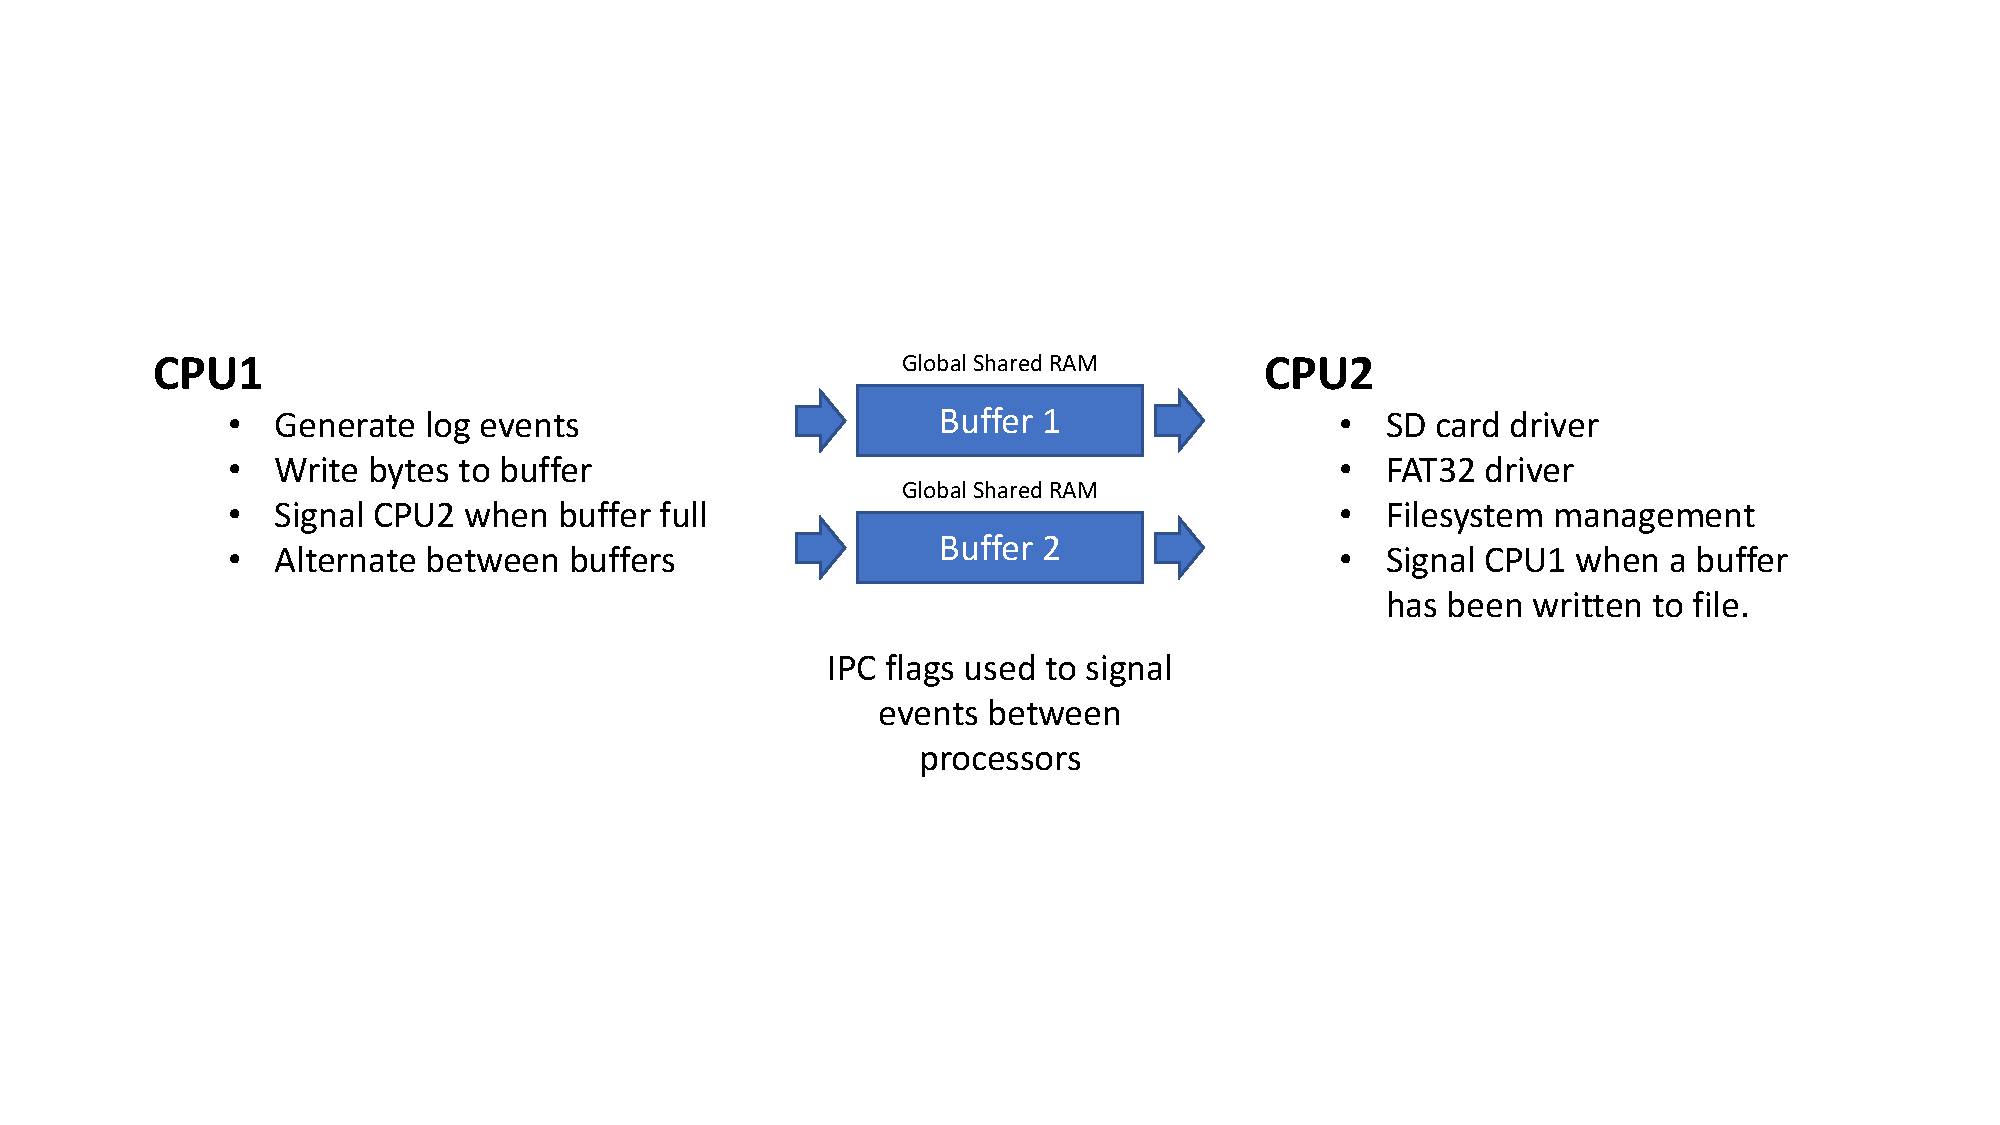
\includegraphics[width=1.0\textwidth]{./figures/logging_structure.pdf}
    \caption{Structure of logging driver.}
    \label{fig:logging_structure}
\end{figure}

\section{External Analog-To-Digital Converter (ADC)}

Driver implementation and optimization.

\section{RS485 Bus}

General RS485 structure with SCI and transceiver. FIFO usage. RTS solution.

\subsection{OADM}

\subsection{OM70}

\subsection{CAN Bus}

General CAN structure. CAN driver from TI.

\subsection{Inverters}

Structure. State machine.

\subsection{BMS}

Structure. Event-based data.

\section{Navigation algorithm}

\section{State Diagram}

\section{Control Law Accelerator (CLA)}

\begin{figure}[H]
    \centering 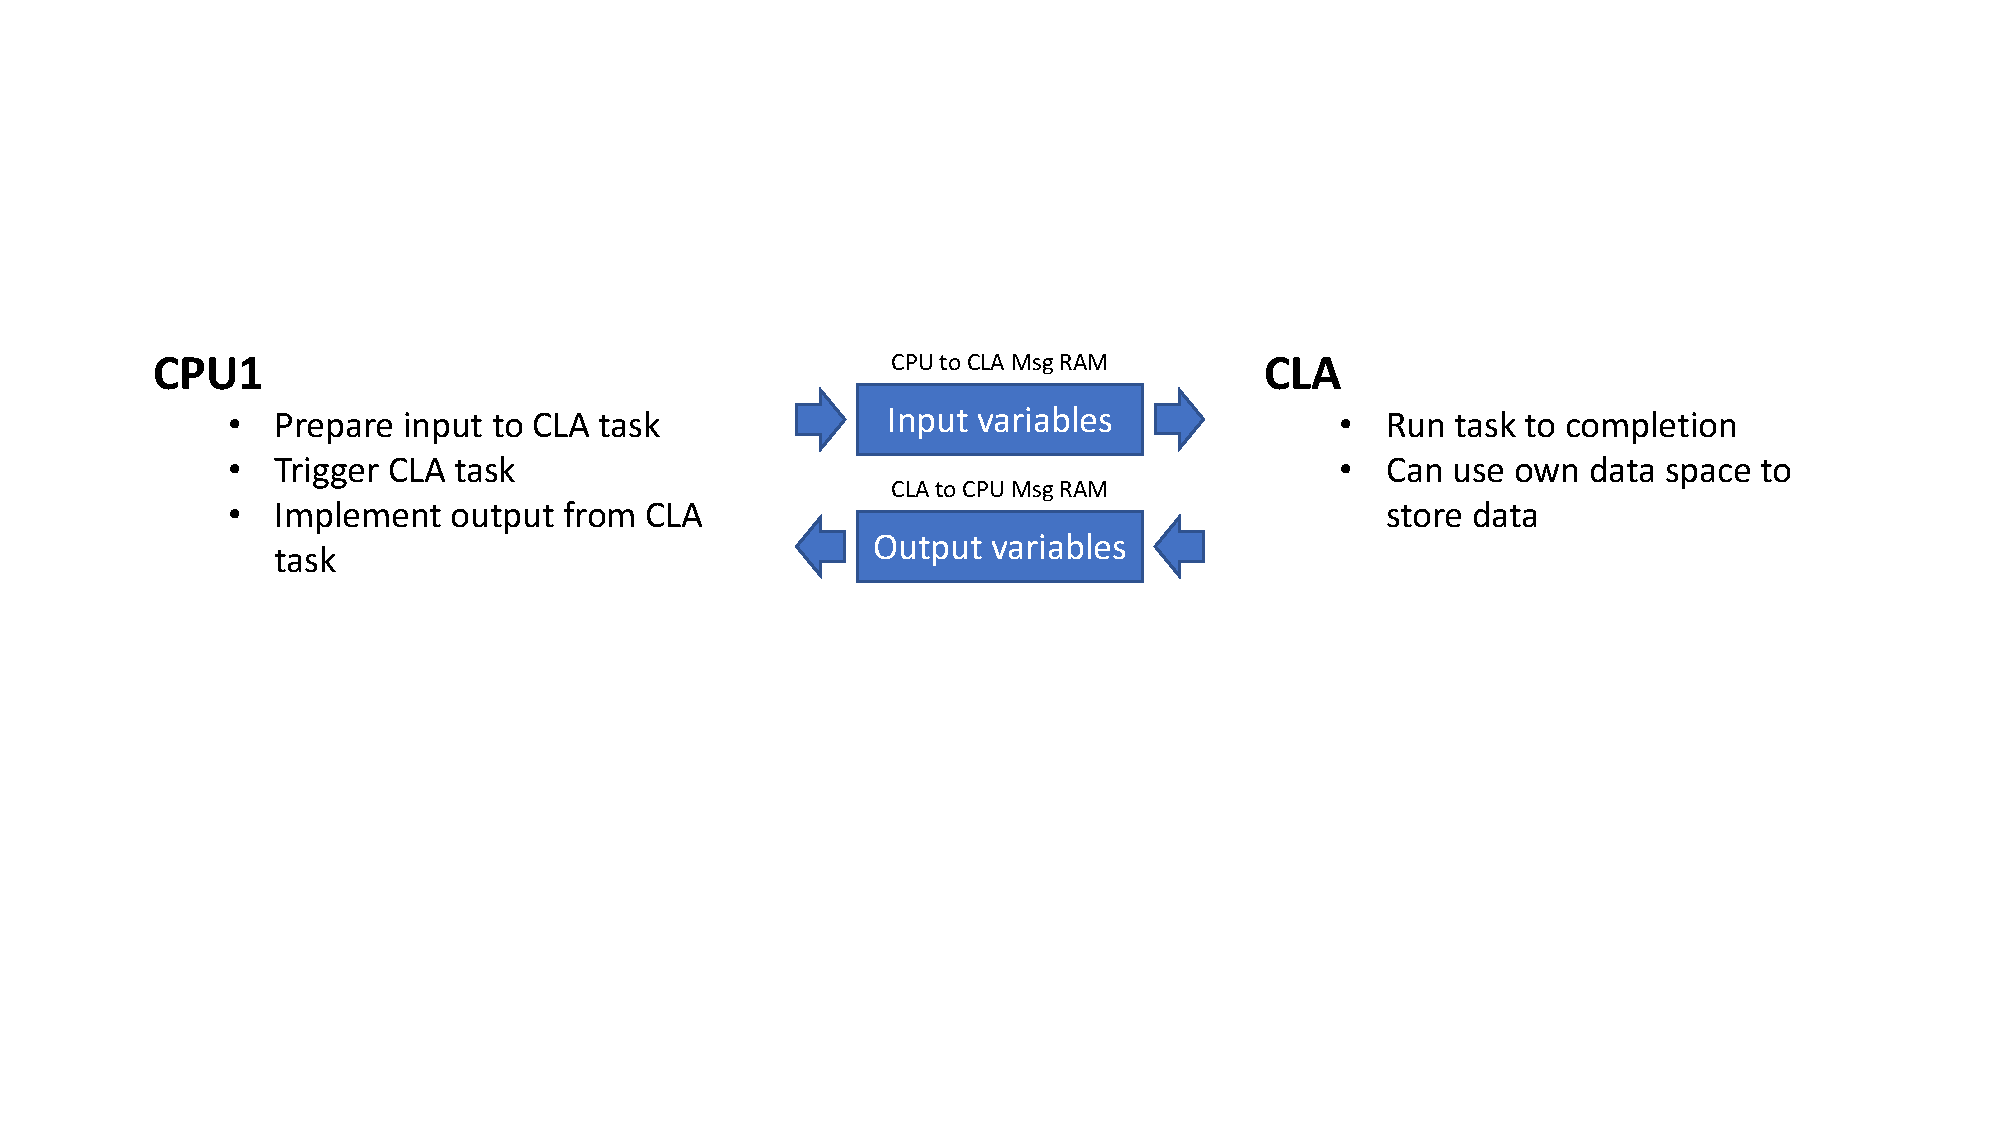
\includegraphics[width=1.0\textwidth]{./figures/CLA_communication.pdf}
    \caption{Communication of inputs ant outputs for CLA tasks.}
    \label{fig:CLA_communication}
\end{figure}

\section{Debugging}

Smaller footprint printf library. Cross-core communication for printing

\section{Unit Testing}
